\documentclass[journal=jpccck,manuscript=article]{achemso}

\usepackage{hyperref}

\usepackage{siunitx}
\DeclareSIUnit\rydberg{Ry}
\usepackage{tikz}
\usepackage{paralist}
\usepackage[version=4]{mhchem}
\usepackage{booktabs}
\usepackage{rotating}
\usepackage{chngcntr}


\author{Pierre Beaujean}
\affiliation[Unamur]
{University of Namur, Theoretical Chemistry Lab, Unit of Theoretical and Structural Physical Chemistry, Namur Institute of Structured Matter, rue de Bruxelles, 61, B-5000 Namur (Belgium)}


\author{Benoît Champagne}
\affiliation[Unamur]
{University of Namur, Theoretical Chemistry Lab, Unit of Theoretical and Structural Physical Chemistry, Namur Institute of Structured Matter, rue de Bruxelles, 61, B-5000 Namur (Belgium)}
\email{benoit.champagne@unamur.be}

\title{Prediction of XPS binding energies for molecules grafted on calcium surfaces\\Supporting information}

\def\dbe{\ensuremath{\Delta\text{BE}}}



\renewcommand{\thetable}{S\arabic{table}}
\renewcommand{\thefigure}{S\arabic{figure}}

\begin{document}
	\maketitle


\begin{figure}[!h]
	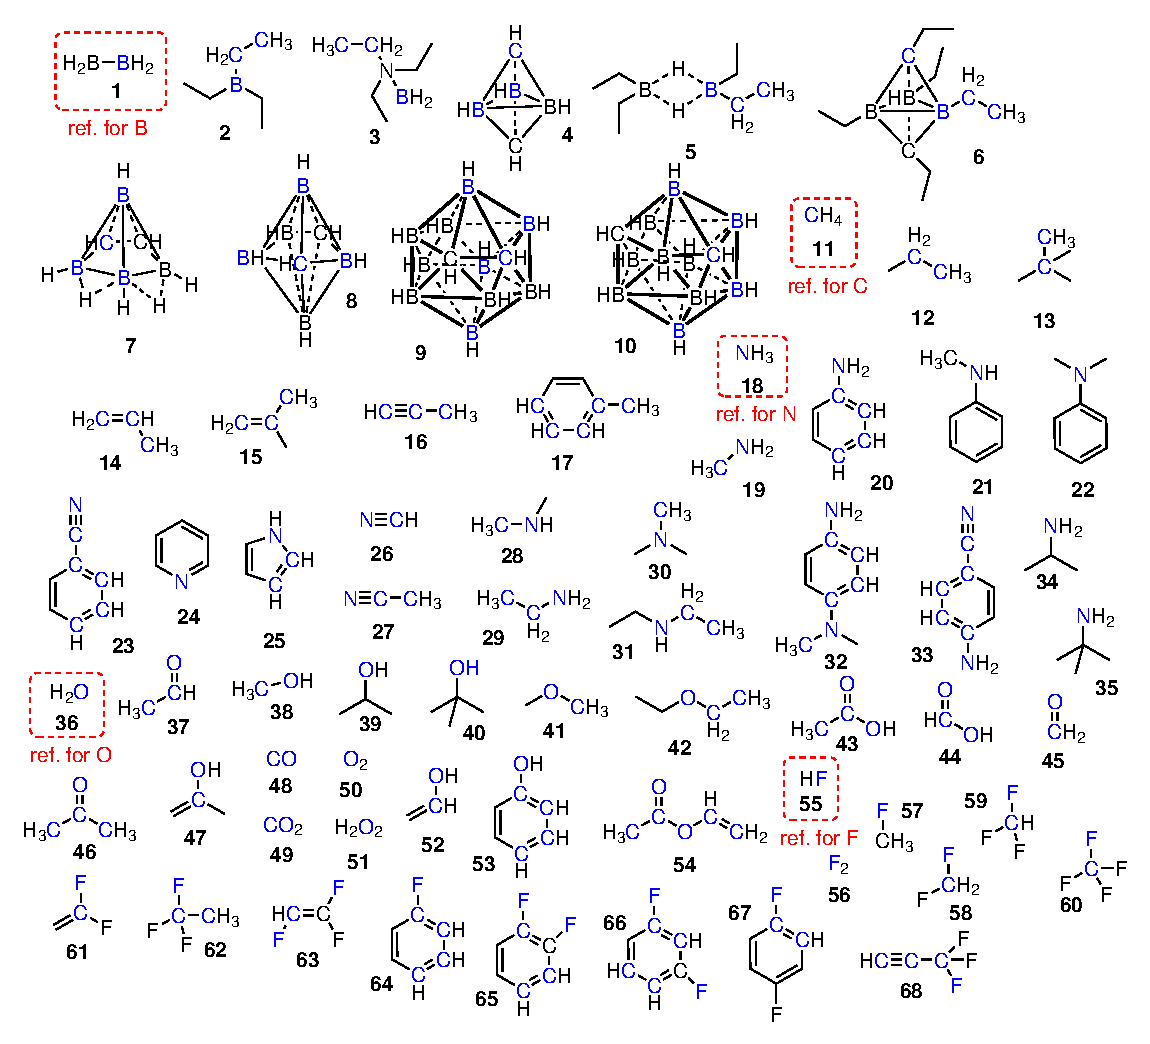
\includegraphics[width=\linewidth]{FigureS1}
	\caption{Evolution of the surface energy for slabs of Ca, CaO, and \ce{CaH2} with increasing thickness ($N$) , as estimated by least-square fit of Eq.~\eqref{eq:surf}. For CaO, the surface energies of (110) and (111) are larger than \SI{1.25}{\joule\per\meter\squared}.}
	\label{fig:surf}
\end{figure}

\begin{figure}[!h]
	\centering
	\includegraphics[width=.8\linewidth]{FigureS2}
	\caption{Comparison between experimental and calculated gas phase \dbe{}, as computed with the SJ (blue) and SJ\textsubscript{n} (orange) protocols on the different atoms, and by shifting the BE by $E_F$ in Eq.~\eqref{eq:xpsbe}. For each of them, the error (as mean $\pm$ standard deviation) for both protocols is given.}
	\label{fig:xps_C185_fermi}
\end{figure}


\begin{figure}[!h]
	\centering
	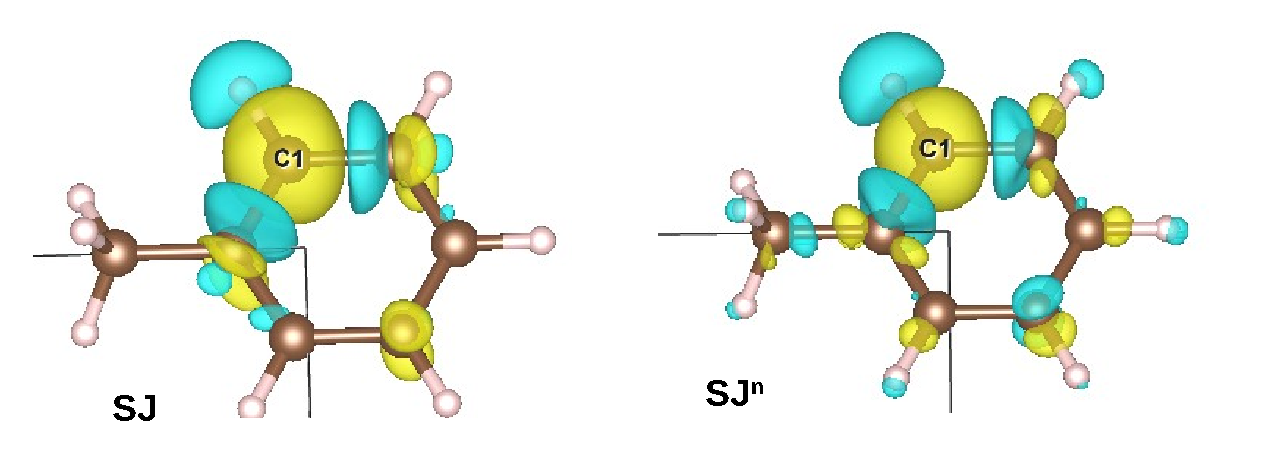
\includegraphics[width=\linewidth]{FigureS3}
	\caption{Impact of the slab thickness (indicated as the number of layers) on the resulting XPS spectra (as computed with the SJ\textsuperscript{n} protocol).}
	\label{fig:slabsthicknessSJn}
\end{figure}


\newcommand{\XPSsa}[3]{
	\begin{figure}[!h]
		\centering
		\includegraphics[width=.8\linewidth]{Figure#1a}
		\includegraphics[width=.8\linewidth]{Figure#1b}
		\caption{Difference (dotted line) between the XPS spectrum before (dashed line) and after (plain line) adsorption for compounds \textbf{#2} (top) and \textbf{#3} (bottom) on the different substrates.}
		\label{fig:spectraXPSads#2#3}
	\end{figure}
}

\XPSsa{S4}{a}{b}
\XPSsa{S5}{c}{d}
\XPSsa{S6}{e}{f}
\XPSsa{S7}{g}{h}
\XPSsa{S8}{i}{j}

\begin{figure}[!h]
	\centering
	\includegraphics[width=.8\linewidth]{FigureS9}
	\caption{XPS spectra (as computed with the SJ\textsuperscript{n} protocol, using $\sigma=\SI{0.6}{\electronvolt}$) of the adsorbates \textbf{h} and \textbf{j} on Ca, CaO and \ce{CaO.H2O}.}
	\label{fig:possSJn}
\end{figure}
	
\end{document}